%%%%%%%%%%%%%%%%%%%%%%%%%%%%%%%%%%%%%%%%%%%%%%%%%%%%%%%%%%%%%%%%%%%%%
% Use the koma-script document style
%\documentclass{scrbook}
%\KOMAoptions{twoside=false} % disable two-side formatting for scrbook
% alternatively, for shorter essay, use the following
\documentclass{scrartcl}
%%%%%%%%%%%%%%%%%%%%%%%%%%%%%%%%%%%%%%%%%%%%%%%%%%%%%%%%%%%%%%%%%%%%%

%%%%%%%%%%%%%%%%%%%%%%%%%%%%%%%%%%%%%%%%%%%%%%%%%%%%%%%%%%%%%%%%%%%%%
% Useful packages
\usepackage{mathtools}
\usepackage{amssymb,bm,bbold}
\usepackage[colorlinks=true]{hyperref}
\usepackage{enumerate}

\usepackage{fullpage}

\usepackage[font=scriptsize,labelfont=bf]{caption}
\usepackage{wrapfig}
\usepackage{tikz}
\usepackage{pgfplots}

%=================================
% pre-defined theorem environments
\usepackage{amsthm}
\newtheorem{theorem}{Theorem}
\newtheorem{lemma}{Lemma}
\newtheorem{proposition}{Proposition}
\newtheorem{corollary}{Corollary}
\newtheorem{definition}{Definition}
\newtheorem*{remark}{Remark}
\newtheorem*{assumption}{Assumption}

\usepackage[framemethod=tikz]{mdframed}
\newmdtheoremenv[
skipabove=\baselineskip,
skipbelow=\baselineskip,
hidealllines=true,
innertopmargin=4pt,
linewidth=4pt,
linecolor=gray!40,
singleextra={
  \draw[line width=3pt,gray!50,line cap=rect] (O|-P) -- +(1cm,0pt);
  \draw[line width=3pt,gray!50,line cap=rect] (O|-P) -- +(0pt,-1cm);
  \draw[line width=3pt,gray!50,line cap=rect] (O-|P) -- +(-1cm,0pt);
  \draw[line width=3pt,gray!50,line cap=rect] (O-|P) -- +(0pt,1cm);
  },
firstextra={
  \draw[line width=3pt,gray!50,line cap=rect] (O|-P) -- +(1cm,0pt);
  \draw[line width=3pt,gray!50,line cap=rect] (O|-P) -- +(0pt,-1cm);
},
secondextra={
  \draw[line width=3pt,gray!50,line cap=rect] (O-|P) -- +(-1cm,0pt);
  \draw[line width=3pt,gray!50,line cap=rect] (O-|P) -- +(0pt,1cm);
}
]{problem}{Problem}

%=================================
% useful commands
\DeclareMathOperator*{\argmin}{arg\,min}
\DeclareMathOperator*{\argmax}{arg\,max}
\DeclareMathOperator*{\supp}{supp}
\DeclareMathOperator*{\minimize}{\mathsf{minimize}}

\def\vec#1{{\ensuremath{\bm{{#1}}}}}
\def\mat#1{\vec{#1}}

%=================================
% convenient notations
\newcommand{\XX}{\mathbb{X}}
\newcommand{\RR}{\mathbb{R}}
\newcommand{\EE}{\mathbb{E}}
\newcommand{\PP}{\mathbb{P}}

\newcommand{\sB}{\mathcal{B}}
\newcommand{\sK}{\mathcal{K}}
\newcommand{\sL}{\mathcal{L}}

\newcommand{\TODO}{\textbf{\textsf{TODO}}}

\usepackage{algpseudocode}
\usepackage{algorithm}

%%%%%%%%%%%%%%%%%%%%%%%%%%%%%%%%%%%%%%%%%%%%%%%%%%%%%%%%%%%%%%%%%%%%%
% Typography, change document font
%\usepackage[libertine,cmintegrals,cmbraces,vvarbb]{newtxmath}
%\usepackage[scaled=0.95]{inconsolata}
\usepackage{lmodern}
\usepackage{charter}
\usepackage[scaled=0.95]{inconsolata}

\title{Intuitions for Optimization}
\author{pluskid}

\begin{document}
\maketitle

\section{Projected Subgradient Descent for Lipschitz Functions}

\subsection{Problem Setup}

\begin{problem}
  Given $f:\RR^n\rightarrow\RR$, and $\sK\subset\RR^n$. Assume $\sK$ is compact and convex, included
  in a Euclidean ball of radius $R$:
  \begin{equation}
    \sK \subset \sB_2(0; R)
  \end{equation}
  and $f$ is convex and $L$-Lipschitz on $\sK$:
  \begin{equation}
    |f(x)-f(y)| \leq L\|x-y\|_2, \quad x,y\in\sK
  \end{equation}
  Find a minimizer of $f$ on $\sK$:
  \[
  \minimize_{x\in\sK} f(x)
  \]
  \label{prob:projected-subgradient-descent}
\end{problem}

\subsection{Algorithm and its Bounds}

\begin{algorithm}
  \caption{Projected Subgradient Descent}
  \begin{algorithmic}
    \State randomly initialize $x^0\in\sK$
    \For{$t\gets 0,\ldots,T-1$}
      \State $y^{t+1}\gets x^{t}-\eta_t g_t$, where $g_t\in\partial f(x^{t})$
      \State $x^{t+1}\gets \Pi_{\sK}(y^{t+1})$
    \EndFor
  \end{algorithmic}
  \label{alg:projected-subgradient-descent}
\end{algorithm}

\begin{theorem}
  Running Algorithm~\ref{alg:projected-subgradient-descent} on Problem~\ref
  {prob:projected-subgradient-descent} for $T$ iterations gives
  \begin{equation}
  \min_{0\leq\tau\leq T}f(x^\tau) - f(x^*) \leq \frac{R^2 + G^2\sum_{t=0}^{T-1}\eta_t^2}{\sum_{t=0}^
  {T-1}\eta_t}
  \label{eq:proj-subgrad-bound}
  \end{equation}
  In general, the optimal bound is around $O(GR/\sqrt{T})$ with stepsizes around $\eta_t\eqsim R/
  (G\sqrt{t})$. That means in order to get an approximate error of $\varepsilon$, we will need to
  run the algorithm for $O(1/\varepsilon^2)$ iterations.
  \label{thm:projected-subgradient-descent}
\end{theorem}

\subsection{Intuitions and Analysis}

\subsubsection{Problem Assumptions}
\label{sec:subgrad-descent-assumption}

We consider the unconstrained case first, i.e. $\sK=\RR^n$. Since $f$ is convex know that $x^*$ is a
minimizer of $f$ if and only if $0\in\partial f (x^*)$. However, without making any extra
assumptions, we have no idea of the behavior of $f$ even in a small neighborhood of $x^*$. Consider
for example $f(x)=C|x|$, with $C>0$ a large constant. Assume we are currently very close to the
optimal $x^*=0$, say $x^t=\varepsilon$, $\varepsilon>0$. $f$ is differentiable at $\varepsilon$, so
the only subgradient is $g_t=C$. Therefore,
\[
  x^{t+1} = x^t - \eta_t g_t
  = \varepsilon - \eta_tC < -\varepsilon, \quad \forall \eta_t > \frac {2\varepsilon} {C}
\]
As we can see, unless the stepsize $\eta_t$ is very tiny, we will overshoot, $f(x^{t+1})>f(x^t)$.
Moreover, if we use a constant stepsize $\eta_t=\eta$, then if $\eta >\varepsilon/C$, we will be
jumping back and forth at $\varepsilon$ and $\varepsilon - \eta C$ indefinitely.

In order to fix this, we need to make additional assumptions. We will see later in the case of
smooth functions, the gradient changes continuously. So we know that at a local neighborhood of the
optimal (gradient is 0), the gradient is also small. But here, we are working with
non-differentiable functions, we will just assume $f$ is $L$-Lipschitz.

Note $f$ being $L$-Lipschitz in $\sK$ implies that $\|g\|_2 \leq L$, $\forall g\in\partial f(x),
\forall x\in\sK$. In order to avoid overshooting, we will have to move with tiny stepsizes.

\subsubsection{Convergence Analysis}
\label{sec:subgrad-lipschitz-analysis}

By the property of subgradient, we have
\begin{equation}
  0\leq f(x^t) - f(x^*) \leq g_t^\top (x^t-x^*) = -g_t^\top (x^*-x^t)
  \label{eq:subgrad-lower-bound-f}
\end{equation}
\begin{wrapfigure}{r}{.35\linewidth}
\centering
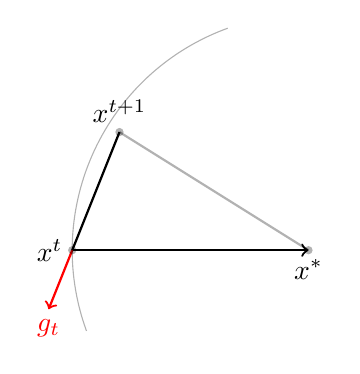
\begin{tikzpicture}[scale=1.5]
  \coordinate [label=left:$x^t$] (Xt) at (-2,0);
  \coordinate [label=below:$x^*$] (Xs) at (0,0);
  \coordinate [label=above:$x^{t+1}$] (Xtp) at (-1.6,1);
  \draw [->,thick] (Xt) -- (Xs);
  \draw [thick] (Xt) -- (Xtp);
  \draw [thick,opacity=.3] (Xs) -- (Xtp);
  \draw [->,thick,red] (Xt) -- (-2.2,-0.5) node [below] {$g_t$};

  \fill [black,opacity=.3] (Xt) circle (1pt);
  \fill [black,opacity=.3] (Xtp) circle (1pt);
  \fill [black,opacity=.3] (Xs) circle (1pt);
  \draw [opacity=.3] ([shift=(110:2)] 0,0) arc (110:200:2);
\end{tikzpicture}
\caption{Demonstration of subgradient descent.}
\label{fig:subgrad-descent-demo}
\end{wrapfigure}
where the left hand side is due to the optimality of $x^*$. This inequality indicates that the
vector $x^*-x^t$ is non-negatively correlated with $-g_t$, the direction of a subgradient descent.

Unlike in the case of differentiable functions, in which we can guarantee that the function values
decreases when moving along the direction of negative gradient with a small enough step size; here
we do not know much about the function values. But as we can see from Figure~\ref
{fig:subgrad-descent-demo}, when the angle between $-g_t$ and $x^*-x^t$ is greater than or equal to $\pi/2$,
we will move away from $x^*$ with any positive step size. However, if $f(x^t)-f(x^*)>0$, i.e. we are
not already at the optimal, the angle is strictly less than $\pi/2$, so if we move with a small
enough step size, we will get closer to $x^*$. Algebraically,
\begin{equation}
\begin{aligned}
  \|x^{t+1}-x^*\|^2 = \|x^{t+1}-x^t + x^t-x^*\|^2
  &= \eta_t^2\|g_t\|^2 + \|x^t-x^*\|^2 - 2\eta_tg_t^\top (x^t-x^*) \\
  &\leq {\color{red}\eta_t^2\|g_t\|^2} + \|x^t-x^*\|^2 - {\color{blue}2\eta_t\left(f(x^t)-f
  (x^*)\right)}
  \label{eq:subgrad-lipschitz-analysis-step}
\end{aligned}
\end{equation}
Since $\|g_t\|\leq L$ by our assumption, the \textcolor{red}{red term} decays quadratically, while
the \textcolor{blue}{blue term} only decays linearly. So when $\eta_t$ is small enough, we will have
$\|x^{t+1}-x^*\|^2 \leq \|x^t-x^*\|^2$. Furthermore, the progress we make by moving towards $x^*$ is
characterized by $f(x^t)-f(x^*)$. So if we are still far away from the optimal, we will be making
quite a lot progress in each step. On the other hand, when $f(x^t)-f(x^*)$ is small, our progress
might be small, but at that point we are already close to the optimal function value $f(x^*)$.

Actually, to get a bound on the algorithm, we can just sum up the previous inequality for all
$t=0,\ldots,T-1$,
\[
  \begin{aligned}
    0\leq\|x^T-x^*\|^2
    &\leq \|x^0-x^*\|^2 + \sum_{t=0}^{T-1}\eta_t^2\|g_t\|^2 - 2\sum_{t=0}^{T-1}\eta_t \left(f(x^t)-f
    (x^*)\right) \\
    &\leq R^2 + G^2\sum_{t=0}^{T-1}\eta_t^2 -2\left(\min_{0\leq\tau\leq T}f(x^\tau) - f
    (x^*)\right)\sum_{t=0}^{T-1}\eta_t
  \end{aligned}
\]
It then implies
\begin{equation}
\min_{0\leq\tau\leq T}f(x^\tau) - f(x^*) \leq \frac{R^2 + G^2\sum_{t=0}^{T-1}\eta_t^2}{\sum_{t=0}^
{T-1}\eta_t}
\end{equation}
which proved Theorem~\ref{thm:projected-subgradient-descent} for the case of unconstrained
optimization ($\sK=\RR^n$).

\subsection{Choosing Step Sizes}

Note \eqref{eq:proj-subgrad-bound} holds for any choices of step sizes $\eta_t$ (though some of them
will give completely trivial bounds). So we could actually optimize the right hand side to get an
``optimal'' bound. To make the problem easier, we choose a fixed stepsize $\eta_t=\eta$ for
$t=0,\ldots,T-1$. So the right hand side becomes
\begin{equation}
  \frac{R^2+G^2T\eta^2}{T\eta} = \frac{R^2}{T\eta} + G^2\eta \geq \frac{2GR}{\sqrt{T}}
  \label{eq:subgrad-bound-fix-eta}
\end{equation}
where the inequality holds with equality when
\begin{equation}
  \eta = \frac{R}{G\sqrt{T}}
\end{equation}
Note the choice of step size depends on several factors:
\begin{description}
  \item[$G$:] As we described in Section~\ref{sec:subgrad-descent-assumption}, large $G$ will force
  us to be careful and move with small step sizes. Our intuition is consistent here.
  \item[$R$:] In our analysis, we only use $R$ to bound $\|x^0-x^*\|$. When $R$ is large, we want to
  use large step size, otherwise we might never reach the optimal in the given time budget $T$.
  Generally when $x^*$ is unknown, $R$ can be bounded by the size of $\sK$ for the case
  of constrained optimization.
  \item[$T$:] The inverse dependency on $T$ can be interpreted as: when having a large time budget,
  we can be a little bit more careful and move slowly.
\end{description}


However, in general, the fact that the step size depends on the total number of iterations is
strange. That means if I want to compute more iterations, I will have to start over again and use a
different step size if I want to bound the performance with formula.

In general, we will prefer to use a decaying learning rate. Specifically, as long as
$\sum_t\eta_t\rightarrow \infty$ and $\sum_t\eta_t^2$ is bounded or approaches infinity at a slower
rate than $\sum_t\eta_t$, \eqref{eq:proj-subgrad-bound} will give a reasonable bound. For example,
take $\eta_t=R/(G\sqrt{t+1})$, since
\[
\begin{aligned}
  \sum_{t=0}^{T-1} \frac{1}{t+1} &\leq 1 + \int_1^{T} \frac{1}{x}\,dx = 1 + \log T \\
  \sum_{t=0}^{T-1} \frac{1}{\sqrt{t+1}} &\geq \int_1^{T+1}\frac{1} {\sqrt{x}}\,dx =
  2\sqrt{T+1}-2
\end{aligned}
\]
Plug-in to \eqref{eq:proj-subgrad-bound}, we get
\begin{equation}
  \min_{0\leq \tau \leq T} f(x^\tau) - f(x^*) \leq GR \frac{1+\log T}{2\sqrt{T+1}-2} \lesssim \frac
  {GR\log T}{\sqrt{T}}
\end{equation}
Comparing with the optimal bound we get with a fixed step size in \eqref{eq:subgrad-bound-fix-eta},
we lose a factor of $\log T$, but our step size does not depend on the total number of iterations any
more.

\subsubsection{Constrained Optimization}

\begin{wrapfigure}{r}{.35\linewidth}
\centering
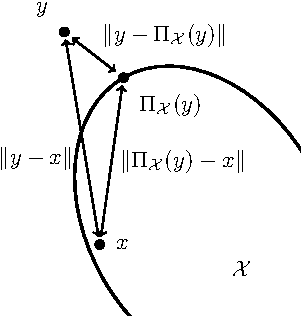
\includegraphics[width=.8\linewidth]{figs/convex-projection}
\caption{Illustration of convex projection. Figure source: S{\'e}bastien Bubeck, \emph{Theory of
Convex Optimization for Machine Learning}.}
\end{wrapfigure}
In the constrained case, we have an extra projection step. However, the same analysis naturally goes
through because projection into convex set is a \emph{contraction}. Specifically, we have the
following lemma.

\begin{lemma}
  Let $\sK\subset\RR^n$ be a closed convex set, let $x\in\sK$ and $y\in\RR^n$. Then
  \begin{equation}
    (x-\Pi_\sK(y))^\top (y-\Pi_\sK(y)) \leq 0
  \end{equation}
  which also implies
  \begin{equation}
    \|x-\Pi_\sK(y)\|^2 + \|y-\Pi_\sK(y)\|^2 \leq \|y-x\|^2
    \label{eq:conv-proj-contraction-0}
  \end{equation}
\end{lemma}

This lemma could be proved with \emph{supporting hyperplane theorem} of convex sets. \eqref
{eq:conv-proj-contraction-0} implies
\[
  \|x-\Pi_{\sK}\|^2 \leq \|y-x\|^2
\]
So if we go back to our analysis in Section~\ref{sec:subgrad-lipschitz-analysis}, the only thing we
need to modify is \eqref{eq:subgrad-lipschitz-analysis-step}. Since $x^*\in\sK$,
\[
  \|x^{t+1}-x^*\|^2 = \|\Pi_\sK(y^{t+1})-x^*\|^2 \leq \|y^{t+1}-x^*\|^2
  = \eta_t^2\|g_t\|^2 + \|x^t-x^*\|^2 - 2\eta_tg_t^\top (x^t-x^*)
\]
and the rest of the analysis follows as before. So for constrained optimization, we get the same
convergence rate as the unconstrained case.

\section{Gradient Descent for Smooth Function}

In this section, we look at smooth functions. Specifically, $f$ is differentiable, and its gradient
$\nabla f$ is Lipschitz continuous. By adding those assumptions, we know better about $f$ than in
the simple Lipschitz case. For example, we know two nearby points should have similar gradients.
In particular, if $x$ is close to the optimal $x^*$, since $\nabla f(x^*)=0$, we know that $\nabla
f(x)$ must be small (close to zero).

\begin{definition}[$\beta$-smooth functions]
A differentiable function $f:\RR^n\rightarrow \RR$ is $\beta$-smooth if its gradient $\nabla f$ is
$\beta$-Lipschitz, that is
\begin{equation}
  \|\nabla f(x)-\nabla f(y)\| \leq \beta \|x-y\|,\quad \forall x,y\in\RR^d
\end{equation}
\end{definition}

\begin{problem}
  Given a convex and $\beta$-smooth function $f:\RR^n\rightarrow\RR$. Find a minimizer of $f$.
  \label{prob:beta-smooth}
\end{problem}

\begin{theorem}
  Solving Problem~\ref{prob:beta-smooth} using gradient descent with step size $\eta_t=1/\beta$ for
  $T$ iterations gives
  \begin{equation}
    f(x^T)-f(x^*) \leq \frac{2\beta \|x_1-x^*\|^2}{T+3}
  \end{equation}
  That means to get an approximation error of $\varepsilon$, we will need to run the algorithm for
  $O(1/\varepsilon)$ iterations.
  \label{thm:beta-smooth}
\end{theorem}
Note we get much faster convergence rate than Problem~\ref{prob:projected-subgradient-descent} by
making more assumptions on $f$. The parameter $\beta$ control the smoothness of $f$: smaller $\beta$
means the gradient of $f$ changes more slowly, and $\eta_t=1/\beta$ means we could make aggressive
movement in each iteration.

\subsection{Sandwiching Smooth Convex Functions}

In the case of convex Lipschitz function, we use the property of subgradient to lower bound $f$.
$\forall x,y\in\RR^n$ and $\forall g\in\partial f(x)$
\[
  f(y) \geq f(x) + g^\top (y-x)
\]
this leads to \eqref{eq:subgrad-lower-bound-f}. And in the proof, we use this to lower bound $f
(x^*)$, making sure that $f(x^t)-f(x^*)$ is controlled, i.e. we are not too far away from the
optimal.

In the scenario of $\beta$-smooth function, we can get the same lower bound, because $\nabla f(x)$
is always the unique subgradient at any point $x$. Moreover, the $\beta$-smoothness gives us an
upper bound:
\[
  f(y) \leq f(x) + \nabla f(x)^\top (y-x) + \frac{\beta}{2}\|y-x\|^2
\]
and this could be used to get a lower bound on the decrement $f(x^t)-f(x^{t+1})$ at each iteration.
Sef Fig.~\ref{fig:lower-and-upper-bnd-smooth-cvx} for an illustration. We state the conclusions
below formally.

\begin{figure}
  \begin{tikzpicture}
    \begin{axis}[width=16cm,height=8cm]
      \addplot[mark=none] {(x+2)^2};
      \addplot[mark=none,red,domain=-2.5:5] {36+12*(x-4)};
      \addplot[mark=none,blue,domain=-1:5] {36+12*(x-4)+3*(x-4)^2};
      \addplot[only marks] coordinates {
        (4,36) (-2,0) (-2,-36) (1,9) (1,27)
      };
      \node at (axis cs:4,36) [anchor=south] {$f(x^t)$};
      \node at (axis cs:-2,0) [anchor=south] {$f(x^*)$};
      \node at (axis cs:-2,-36) [anchor=south east] {$f_L(x^*)$};
      \node at (axis cs:1,9) [anchor=south east] {$f_L(x^{t+1})$};
      \node at (axis cs:1,27) [anchor=south west] {$f_U(x^{t+1})$};

      \addplot[mark=none,dashed,red] coordinates {
        (-2,0) (-2,-36)
      };
      \addplot[mark=none,dashed,blue] coordinates {
        (1,9) (1,27)
      };
    \end{axis}
  \end{tikzpicture}
  \caption{Illustration of a convex $\beta$-smooth function $f(x)$, with its lower bound $f^L(x)=f
  (x_0)+\langle \nabla f(x_0),x-x_0\rangle$ and upper bound $f^U(x)=f(x_0)+\langle \nabla f(x_0),
  (x-x_0)\rangle + 0.5\beta\|x-x_0\|^2$. The lower bound makes sure $f (x^t)$ is not too far away
  from $f (x^*)$, while
  the upper bound makes sure some progress $f(x^t)-f(x^{t+1})$ are made in each iteration.}
  \label{fig:lower-and-upper-bnd-smooth-cvx}
\end{figure}

\begin{lemma}
  Assume $f:\RR^n\rightarrow \RR$ is $\beta$-smooth, then $\forall x,y\in\RR^n$
  \[
  |f(y)-f(x)- \langle \nabla f(x), y-x\rangle | \leq \frac{\beta}{2}\|y-x\|^2
  \]
\end{lemma}
\begin{proof}
By the fundamental theorem for line integrals,
\[
  f(y) = f(x) + \int_{0}^1 \langle \nabla f(x + t(y-x)), y-x\rangle dt
\]
Plugin $f(y)-f(x)$,
\[
  \begin{aligned}
  |f(y)-f(x)- \langle \nabla f(x), y-x\rangle | \leq \frac{\beta}{2}\|y-x\|^2
  &= \left| \int_0^1 \langle \nabla f(x+t(y-x))-\nabla f(x), y-x\rangle dt \right| \\
  &\leq \|y-x\|\int_0^1 \|\nabla f(x+t(y-x))-\nabla f(x)\| dt \\
  &\leq \|y-x\|\int_0^1 \beta t\|y-x\|dt \\
  &=\frac{\beta}{2}\|y-x\|^2
  \end{aligned}
\]
\end{proof}

If we further know that $f$ is convex, combining the lower bound from the first order condition of
convexity, we get both lower bound and upper bound
\begin{equation}
  0 \leq f(y) - f(x) - \langle \nabla f(x), y-x\rangle \leq \frac{\beta}{2}\|y-x\|^2
  \label{eq:beta-smooth-lower-upper-bnd-0}
\end{equation}
See again Fig.~\ref{fig:lower-and-upper-bnd-smooth-cvx} for an illustration.

\subsection{Convergence Analysis and Tighter Sandwiching}

To analyze the convergence, let $\Delta_t=f(x^t)-f(x^*)$ be the suboptimality gap at $x^t$. Let
$y=x^*$, and $x=x^t$ in \eqref{eq:beta-smooth-lower-upper-bnd-0}, and using the lower bound, we can
upper bound $\Delta_t$ by
\begin{equation}
  \Delta_t = f(x^t)-f(x^*) \leq -\langle \nabla f(x^t), x^*-x^t\rangle
  \leq \|\nabla f(x^t)\|\|x^*-x^t\| \leq R\|\nabla f(x^t)\|
  \label{eq:beta-smooth-grad-analysis-0}
\end{equation}
where we define
\begin{equation}
  R=\max_{1\leq t\leq T}\|x^*-x^t\|
\end{equation}
On the other hand, using the upper bound in \eqref{eq:beta-smooth-lower-upper-bnd-0} by letting
$y=x^{t+1}$ and $x=x^t$, we could lower bound $\Delta_t-\Delta_{t+1}$ by
\[
\begin{aligned}
  \Delta_t-\Delta_{t+1} = f(x^t)-f(x^{t+1})
  &\geq -\langle \nabla f(x^t), x^{t+1}-x^t\rangle - \frac{\beta}{2}\|x^{t+1}-x^t\| \\
  &= \left(\eta_t - \frac{\beta\eta_t^2}{2}\right) \|\nabla f(x^t)\|^2
\end{aligned}
\]
Naturally, we want to maximize the lower bound, so the step size is chosen to be
$\eta_t = 1/\beta$. Combining with \eqref{eq:beta-smooth-grad-analysis-0}, we get
\begin{equation}
   \Delta_t - \Delta_{t+1}\geq \frac{1}{2\beta}\|\nabla f(x^t)\|^2
   \geq \frac{1}{2\beta R^2}\Delta_t^2
 \end{equation}
 Note the right hand side is non-negative, so $\Delta_t\geq \Delta_{t+1}$. To solve this recursion,
 divide both side by $\Delta_t\Delta_{t+1}$:
 \begin{equation}
   \frac{1}{\Delta_{t+1}} - \frac{1}{\Delta_t} \geq \frac{1}{2\beta R^2}\frac{\Delta_t}{\Delta_
   {t+1}} \geq \frac{1}{2\beta R^2}
 \end{equation}
 Sum the recursion for $t=2,\ldots,T$, we get
 \[
 \frac{1}{\Delta}_T \geq \frac{T-1}{2\beta R^2} + \frac{1}{\Delta_1}
 \geq \frac{T+3}{2\beta R^2}
 \]
 where the last inequality is because $\Delta_1$ can be controlled by the upper bound in
 \eqref {eq:beta-smooth-lower-upper-bnd-0}. Let $x=x^*$ and $y=x^1$, notice $\nabla f(x^*)=0$,
 \[
 \Delta_1 = f(x^1)-f(x^*) \leq \frac{\beta}{2}\|x^1-x^*\|^2 \leq \frac{\beta R^2}{2}
 \]

At this point, we almost proved Theorem~\ref{thm:beta-smooth}, except that we have to control $R$.
In the following, we will show that $\|x^t-x^*\|$ is actually decreasing at each iteration, and
bound $R$ by $\|x^1-x^*\|$. Recall in the case of subgradient descent, we use the linear lower bound
of the function by the subgradient to construct the inequality in \eqref
{eq:subgrad-lipschitz-analysis-step}. That inequality shows that when $\eta_t$ is small enough,
because the quadratic term decays faster, we get $\|x^{t+1}-x^*\|^2\leq \|x^t-x^*\|^2$. However, in
the case here, since $\eta_t=1/\beta$, especially when $\beta$ is small, we could be moving with
very large step size. So the argument is no longer useful here.

To properly bound $R$, we will need to get a better lower bound of $f$ than in \eqref
{eq:beta-smooth-lower-upper-bnd-0}.
Actually, combining
convexity and $\beta$-smoothness, the lower bound in \eqref{eq:beta-smooth-lower-upper-bnd-0} could
be improved. Consider the extreme case when $f(x)$ is a linear function, then the lower bound is
actually tight. In this case, we also have $\nabla f(x)=\nabla f(y)$. However, if $f(x)$ is not
linear, $\nabla f(x)\neq \nabla f(y)$, we might observe a non-zero gap between $f(x)$ and its linear
lower bound. It is also intuitive that the gap might be larger when the gradient $\nabla f(y)$
changed a lot from $\nabla f(x)$, so we are thinking about getting a better lower bound using the
quantity $\|\nabla f(x)-\nabla f(y)\|$.

\begin{lemma}
  Let $f:\RR^n\rightarrow\RR$ be a convex and $\beta$-smooth function, then $\forall x,y\in\RR^n$
  \begin{equation}
  \frac{1}{2\beta}\|\nabla f(x)-\nabla f(y)\|^2
  \leq f(y) - f(x) - \langle \nabla f(x), y-x\rangle
  \leq \frac {\beta} {2}\|y-x\|^2
  \label{eq:beta-smooth-lower-upper-bnd-1}
  \end{equation}
\end{lemma}
\begin{proof}
  In order to invite both $\nabla f(x)$ and $\nabla f(y)$ into play, we consider a third point
  $z\in\RR^n$, and approximate $f(z)$ from below by $\nabla f(y)$ and from above by $\nabla f(x)$,
  respectively. Using \eqref{eq:beta-smooth-lower-upper-bnd-0}
  \[
  \begin{aligned}
    f(z) - f(x) - \langle \nabla f(x), z-x\rangle &\geq 0\\
    f(z) - f(y) - \langle \nabla f(y), z-y\rangle &\leq \frac{\beta}{2}\|z-y\|^2
  \end{aligned}
  \]
  Multiply the first inequality by $-1$ and sum the two inequalities, we get
  \[
  f(x)-f(y)+\langle \nabla f(x), z-x\rangle - \langle \nabla f(y),z-y\rangle \leq \frac{\beta}
  {2}\|z-y\|^2
  \]
  Re-write the inequality by moving the quantity we want to lower bound to the right,
  \[
   \langle \nabla f(x), z-y\rangle - \langle \nabla f(y),z-y\rangle - \frac{\beta}{2}\|z-y\|^2\leq f
   (y)-f (x)-\langle \nabla f (x),y-x\rangle
  \]
  Inspecting the left hand side, if we let $z=y+\alpha (\nabla f(y)-\nabla f(x))$ for any
  $\alpha\in\RR$, we get
  \[
  \left(\alpha - \frac{\alpha^2\beta}{2}\right)\|\nabla f(y)-\nabla f(x)\|^2\leq f (y)-f (x)-\langle
  \nabla f
  (x),y-x\rangle
  \]
  Since the lower bound is a quadratic function in $\alpha$, we can maximize the lower bound by
  taking $\alpha = 1/\beta$. And the conclusion follows.
\end{proof}

With the improved lower bound of $f$ in \eqref{eq:beta-smooth-lower-upper-bnd-1}, we can now bound
$R$ by showing that
\[
  \begin{aligned}
    \|x^{t+1}-x^*\|^2
    &=\|x^t-x^*\|^2 + \frac{1}{\beta^2}\|\nabla f(x^t)\|^2 - \frac{2}{\beta}\langle \nabla f(x^t),
    x^t-x^*\rangle \\
    &\leq \|x^t-x^*\|^2 + \frac{1}{\beta^2}\|\nabla f(x^t)\|^2
    - \frac{2}{\beta}\left(f(x^t)-f(x^*) + \frac{1}{2\beta}\|\nabla f(x^t)-\nabla f(x^*)\|^2\right)
    \\
    &\leq \|x^t-x^*\|^2 + \frac{1}{\beta^2}\|\nabla f(x^t)\|^2 - \frac{2}{\beta}\times \frac{1}
    {2\beta}\|\nabla f(x^t)\|^2 \\
    & = \|x^t-x^*\|^2
  \end{aligned}
\]
Therefore, $R\leq \|x^1-x^*\|$, which conclude the proof of Theorem~\ref{thm:beta-smooth}. Note if
we move with a step size slightly larger than $1/\beta$, the proof above will no longer be valid.

%\bibliographystyle{alpha}
%\bibliography{bibfile}

\end{document}
